\section{Locked Synthetic Results}

All five preregistered gates passed. Here ``MOSAIC-transfer'' denotes the
capacity-transfer fallback used before the transform-exact refinement. The
independent replay recomputed 128,000
exact external risks and 128,000 deployment labels from 64,000 method-level
receipts with zero mismatch.  Figure~\ref{fig:confirmation} reports every
registered deployment rule in the two primary cells; the population oracle is
omitted from the bars because it is a feasibility diagnostic rather than an
implementable method.

\begin{figure*}[t]
  \centering
  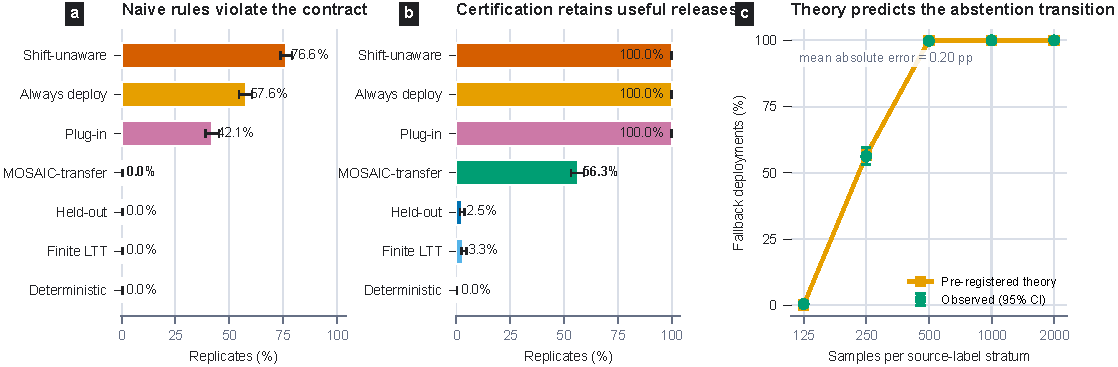
\includegraphics[width=\textwidth]{figures/figure2_mosaic_confirmation.pdf}
  \caption{Hash-locked confirmation with 1,000 independent certification
  tables per cell.  Error bars are exact 95\% Clopper--Pearson intervals.
  (a) At the hard safety boundary, plug-in continuum selection falsely accepts
  42.1\% of tables, whereas MOSAIC-transfer abstains and records no false acceptance.
  Ignoring registered shift is worse.  (b) In the feasible retention cell,
  MOSAIC-transfer safely deploys on 56.3\% of tables, compared with 2.5\% for a held-out
  fixed-channel certificate, 3.3\% for finite LTT, and 0\% for deterministic
  MOSAIC. Non-certifying rules happen to be safe in this easier cell but fail
  in panel (a).  (c) The deployment transition follows the theory curve frozen
  before outcomes (mean absolute error 0.20 percentage points).}
  \label{fig:confirmation}
\end{figure*}

\begin{table}[t]
\centering
\small
\setlength{\tabcolsep}{3.1pt}
\begin{tabular}{lrrr}
\hline
Rule & Deploy & False accept & Safe deploy \\
\hline
\multicolumn{4}{l}{\emph{Hard safety boundary, $n=125$}} \\
Always deploy        & 100.0 & 57.6 & 42.4 \\
Shift-unaware MOSAIC &  80.3 & 76.6 &  3.7 \\
Plug-in continuum    &  73.7 & 42.1 & 31.6 \\
\textbf{MOSAIC-transfer} & 0.0 & \textbf{0.0} & 0.0 \\
\hline
\multicolumn{4}{l}{\emph{Retention regime, $n=250$}} \\
Held-out fixed       &   2.5 &  0.0 &  2.5 \\
Finite LTT           &   3.3 &  0.0 &  3.3 \\
Deterministic MOSAIC &   0.0 &  0.0 &  0.0 \\
\textbf{MOSAIC-transfer} & \textbf{56.3} & 0.0 & \textbf{56.3} \\
\hline
\end{tabular}
\caption{Primary registered rates (\%).  Each row uses the same 1,000 tables
within a cell.  ``False accept'' means deployed while violating at least one
exact external privacy or utility contract.}
\label{tab:primary}
\end{table}

The safety contrast is paired: plug-in selection has 421 false acceptances
that MOSAIC-transfer avoids and there are no reverse discordances. The paired rate
difference is 42.1 points (bootstrap 95\% interval $[39.0,45.2]$; exact
McNemar $p=3.69\times10^{-127}$). Across all eight registered fallback cells,
including 8,000 independently sampled certification tables, no accepted
release violates the exact external contract.  This is finite-run evidence
consistent with the theorem, not a replacement for its $1-\delta$ guarantee.

In the retention cell, MOSAIC-transfer improves safe deployment over held-out
certification by 53.8 points ($[50.6,56.9]$), finite LTT by 53.0 points
($[49.9,56.1]$), and deterministic MOSAIC by 56.3 points ($[53.2,59.3]$);
all paired exact $p$-values are below $2.1\times10^{-158}$.  The stochastic
comparison is essential: no deterministic channel satisfies the same
finite-sample contract in this cell. Fallback deployment rises from 0.5\% at
$n=125$ to 56.3\% at $n=250$, 99.8\% at $n=500$, and 100\% at $n\geq1000$.
The preregistered local power approximation has 0.20-point mean absolute error
over these five sizes and 0.44-point error at the primary size.  Its active-set
and two-step gradient-stability diagnostics pass at every registered point.
